\section{镜面反射与透射}\label{sec:镜面反射与透射}

绝对光滑表面上光的特性较容易用物理和几何光学模型分析刻画。
这些表面展现出入射光的完美镜像反射和透射;
对于给定的方向${\bm\omega}_{\mathrm{i}}$,
所有光都散射到单个出射方向${\bm\omega}_{\mathrm{o}}$.
对于镜面反射,该出射方向和法线所成角与入射方向相同:
\begin{align*}
    \theta_{\mathrm{i}}=\theta_{\mathrm{o}}\, ,
\end{align*}
且其中$\varphi_{\mathrm{o}}=\varphi_{\mathrm{i}}+\pi$.
对于透射,我们也有$\varphi_{\mathrm{o}}=\varphi_{\mathrm{i}}+\pi$,
且出射方向$\theta_{\mathrm{t}}$由斯涅尔定律给出,
它将折射方向与曲面法线$\bm n$的夹角$\theta_{\mathrm{t}}$与
入射光线与曲面法线$\bm n$的夹角$\theta_{\mathrm{i}}$联系起来
(本章末的习题之一是用光学的费马原理推导斯涅尔定律)。
斯涅尔定律基于入射光线所在介质的\keyindex{折射率}{index of refraction}{}和
要进入的介质的折射率。折射率描述了光在特定介质中相比在真空中传播要慢多少。
我们用希腊字母$\eta$表示折射率,读作“eta”。斯涅尔定律是
\begin{align}
    \label{eq:8.2}
    \eta_{\mathrm{i}}\sin\theta_{\mathrm{i}}=\eta_{\mathrm{t}}\sin\theta_{\mathrm{t}}\, .
\end{align}

通常,折射率随波长变化。因此,在两种不同介质界面上入射光通常散射到多个方向,
该效应称为\keyindex{色散}{dispersion}{}。
当入射白光被棱镜分出光谱成分时可以观察到该效应。
图形学中的通行做法是忽略该波长依赖性,
因为该效应通常对视觉准确性并不关键且忽略它能极大简化光传输计算。
可选地,可以在有色散物体的环境中追踪多束光路(例如一系列离散波长)。
第\refchap{光传输I:表面反射}末的“扩展阅读”一节有关于该话题的更多信息指引。
\begin{figure}[htbp]
    \centering
    \subfloat[镜面反射]{\includegraphics[width=0.75\linewidth]{chap08/dragon-specular-reflect.png}\label{fig:8.4.1}}\\
    \subfloat[镜面透射]{\includegraphics[width=0.75\linewidth]{chap08/dragon-specular-transmit.png}\label{fig:8.4.2}}
    \caption{用(1)完美镜面反射和(2)完美镜面折射渲染的龙模型。图像(2)排除了
        内外反射的影响;导致的能量损失产生了显眼的暗区(感谢Christian Schüller提供模型)。}
    \label{fig:8.4}
\end{figure}

\reffig{8.4}展示了完美镜面反射和透射的效果。

\subsection{菲涅尔反射率}\label{sub:菲涅尔反射率}
除了反射和透射方向,还有必要计算反射或透射的入射光占比。
为了物理上准确反射或折射,该项依赖于方向,而不能用每个表面的缩放常数表征。
\keyindex{菲涅耳方程}{Fresnel equations}{}
\sidenote{译者注:得名于法国物理学家奥古斯丁·菲涅耳(Augustin-Jean Fresnel)。}描述了
表面上反射光的量;它们是麦克斯韦方程在光滑表面上的解。

给定折射率和入射光与曲面法线所成角度,菲涅耳方程
指定了材料对两种不同偏振状态的入射照明相应的反射率。
因为偏振的视觉效果在大多数环境下是受限的,
所以在pbrt中我们将作出光是无偏振的常用假设;
即光波是随机朝向的。有了该简化假设,菲涅尔反射率就是
平行和垂直偏振项的均方。

此刻有必要指出几个重要材料类别的差异:
\begin{enumerate}
    \item 第一类是\keyindex{介电质}{dielectric}{},
          是不会导电的材料。它们有实数值的折射率(通常在范围1-3内)且
          透射\footnote{注意介电质可能充满能吸收大部分或所有透射光的粒子(例如石油)。
              像水那样的介电质也能通过添加离子使之导电而变成电解质溶液。
              这两方面都和材料本身划分为介电质或导体无关。}一部分入射照明。
          介电质的例子有玻璃、矿油、水和空气。
    \item 第二类组成是\keyindex{导体}{conductor}{}例如金属。
          价电子可以自由地在原子晶格中移动,允许电流从一个地方流到另一处。
          当导体受到电磁辐射例如可见光时,这一基本的原子属性就会转化为完全不同的特性:
          该材料是不透明的并反射回大部分照明。一部分光也透射进导体内部并被迅速吸收:
          总吸收通常发生在材料表面0.1$\mu\mathrm{m}$内,因此只有极薄的金属膜才能透射足够的光量。
          我们在pbrt中忽略该效应而只建模导体的反射部分。与介电质相反,
          导体有复数值的折射率$\bar{\eta}=\eta+\mathrm{i}k$.
    \item \keyindex{半导体}{semiconductor}{}例如硅或锗是本书中我们不予考虑的第三类。
\end{enumerate}

导体和介电质都由同一组菲涅尔方程表征。
尽管如此,我们更喜欢为介电质创建特殊的求值函数,
这样当折射率保证为实数值时,这些方程会取特别简单的形式。

\begin{table}[htbp]
    \centering
    \begin{tabular}{ll}
        \toprule
        \textbf{介质}  & \textbf{折射率}$\eta$ \\
        \midrule
        真空           & 1.0                   \\
        海平面上的空气 & 1.00029               \\
        冰             & 1.31                  \\
        水(20℃)      & 1.333                 \\
        熔融石英       & 1.46                  \\
        玻璃           & 1.5-1.6               \\
        蓝宝石         & 1.77                  \\
        钻石           & 2.42                  \\
        \bottomrule
    \end{tabular}
    \caption{各种物体的折射率,给出了光在真空中的速度与
        光在介质中的速度的比值。它们通常是与波长相关的量;
        这些值是在可见波长上的均值。}
    \label{tab:8.1}
\end{table}

为了计算两种介电质界面处的菲涅尔反射率,我们
需要知道这两种介质的折射率。\reftab{8.1}有许多介电质的折射率。
介电质的菲涅尔反射率公式是
\begin{align*}
    r_{\parallel} & =\frac{\eta_{\mathrm{t}}\cos\theta_{\mathrm{i}}-\eta_{\mathrm{i}}\cos\theta_{\mathrm{t}}}{\eta_{\mathrm{t}}\cos\theta_{\mathrm{i}}+\eta_{\mathrm{i}}\cos\theta_{\mathrm{t}}}\, , \\
    r_{\perp}     & =\frac{\eta_{\mathrm{i}}\cos\theta_{\mathrm{i}}-\eta_{\mathrm{t}}\cos\theta_{\mathrm{t}}}{\eta_{\mathrm{i}}\cos\theta_{\mathrm{i}}+\eta_{\mathrm{t}}\cos\theta_{\mathrm{t}}}\, ,
\end{align*}
其中$r_{\parallel}$是平行偏振光的菲涅尔反射率,
$r_{\perp}$是垂直偏振光的反射率,$eta_{\mathrm{i}}$和$\eta_{\mathrm{t}}$是
入射和透射介质的折射率,$\bm\omega_{\mathrm{i}}$和$\bm\omega_{\mathrm{t}}$是
入射和透射方向。$\bm\omega_{\mathrm{t}}$由斯涅尔定律算出(见\refsub{镜面透射})。

余弦项应该大于或等于零;出于计算这些值的目的,
当计算$\cos\theta_{\mathrm{i}}$和$\cos\theta_{\mathrm{t}}$时,
几何法线应该分别翻转到和$\bm\omega_{\mathrm{i}}$或$\bm\omega_{\mathrm{t}}$同侧。

对于非偏振光,菲涅尔反射率是
\begin{align*}
    F_{\mathrm{r}}=\frac{1}{2}(r_{\parallel}^2+r_{\perp}^2)\, .
\end{align*}

因为能量守恒,介电质传输的能量为$1-F_{\mathrm{r}}$.

函数\refvar{FrDielectric}{()}为介电质材料和非偏振光计算菲涅尔反射率公式。
量$\cos\theta_{\mathrm{i}}$作为参数{\ttfamily cosThetaI}传入。
\begin{lstlisting}
`\initcode{BxDF Utility Functions}{=}`
`\refvar{Float}{}` `\initvar{FrDielectric}{}`(`\refvar{Float}{}` cosThetaI, `\refvar{Float}{}` etaI, `\refvar{Float}{}` etaT) {
    cosThetaI = `\refvar{Clamp}{}`(cosThetaI, -1, 1);
    `\refcode{Potentially swap indices of refraction}{}`
    `\refcode{Compute cosThetaT using Snell's law}{}`
    `\refvar{Float}{}` Rparl = ((etaT * cosThetaI) - (etaI * cosThetaT)) /
                  ((etaT * cosThetaI) + (etaI * cosThetaT));
    `\refvar{Float}{}` Rperp = ((etaI * cosThetaI) - (etaT * cosThetaT)) /
                  ((etaI * cosThetaI) + (etaT * cosThetaT));
    return (Rparl * Rparl + Rperp * Rperp) / 2;
}
\end{lstlisting}

为了求得折射角的余弦{\ttfamily cosThetaT},
首先需要确定入射方向是在介质的外面还是里面,这样才能恰当解释两个折射率。

入射角余弦的符号表明了入射光在介质的哪一侧(\reffig{8.5})。
如果余弦在0到1间,则光线在外侧,如果在-1到0间,则光线在内侧。
调整参数{\ttfamily etaI}和{\ttfamily etaT}使得{\ttfamily etaI}
是入射介质的折射率,这样保证了{\ttfamily cosThetaI}非负。

\begin{figure}[htbp]
    \centering
    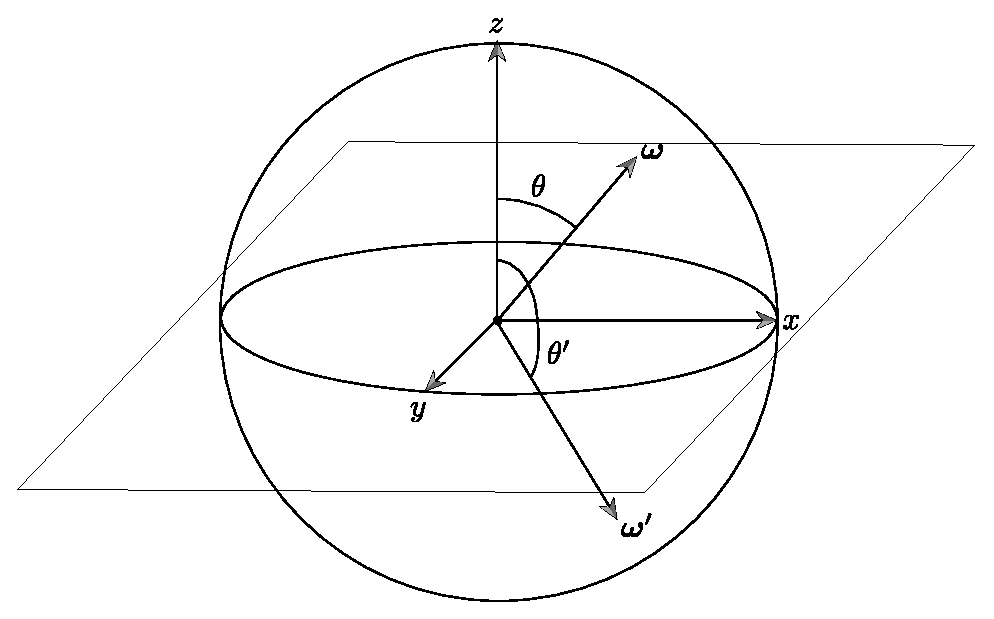
\includegraphics[width=0.7\linewidth]{chap08/BSDFanglegivesinout.eps}
    \caption{方向$\bm\omega$和几何曲面法线间夹角$\theta$的余弦
        表明方向是指向表面外侧(和法线在同一半球)还是表面内侧。
        在标准反射坐标系中,该测试只要求检查方向向量的$z$分量。
        这里,$\bm\omega$在上半球,取正值余弦,而${\bm\omega}'$在下半球。}
    \label{fig:8.5}
\end{figure}

\begin{lstlisting}
`\initcode{Potentially swap indices of refraction}{=}`
bool entering = cosThetaI > 0.f;
if (!entering) {
    std::swap(etaI, etaT);
    cosThetaI = std::abs(cosThetaI);
}
\end{lstlisting}

一旦确定折射率,我们就能用斯涅尔定律(\refeq{8.2})计算
透射方向和曲面法线夹角的正弦$\sin\theta_{\mathrm{t}}$.
最后,用恒等式$\sin^2\theta+\cos^2\theta=1$求得该角的余弦。
\begin{lstlisting}
`\initcode{Compute cosThetaT using Snell's law}{=}`
`\refvar{Float}{}` sinThetaI = std::sqrt(std::max((`\refvar{Float}{}`)0,
                                     1 - cosThetaI * cosThetaI));
`\refvar{Float}{}` sinThetaT = etaI / etaT * sinThetaI;
`\refcode{Handle total internal reflection}{}`
`\refvar{Float}{}` cosThetaT = std::sqrt(std::max((`\refvar{Float}{}`)0,
                                     1 - sinThetaT * sinThetaT));
\end{lstlisting}

当从一种介质传播到另一种折射率更低的介质时,入射角接近掠角的光不能进入另一介质。
发生该现象的最大角称为\keyindex{临界角}{critical angle}{};
当$\theta_{\mathrm{i}}$大于临界角时,发生\keyindex{全内反射}{total internal reflection}{reflection反射},
所有光都被反射。这里通过$\sin\theta_{\mathrm{t}}$大于1检测到该情况;
此时不需要菲涅尔方程。
\begin{lstlisting}
`\initcode{Handle total internal reflection}{=}`
if (sinThetaT >= 1)
    return 1;
\end{lstlisting}

我们现在聚焦一般情况下的复数折射率$\bar{\eta}=\eta+\mathrm{i}k$,
其中一些入射光被材料部分吸收并变为热量。
除了实部,一般菲涅尔公式现在也依赖于虚部$k$,
称为\keyindex{吸收系数}{absorption coefficient}{}。

\reffig{8.6}展示了金的折射率和吸收系数图示。两者都是与波长相关的量。
pbrt发行版中目录{\ttfamily scenes/spds/metals}下有各种金属的$\eta$与$k$与波长相关的数据。
下章的\reffig{9.4}展示了用金属材料渲染的模型。
\begin{figure}[htbp]
    \centering
    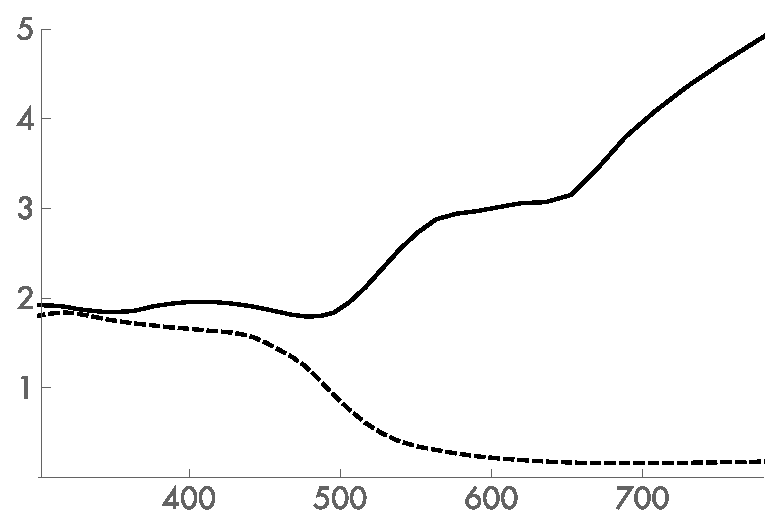
\includegraphics[width=0.7\linewidth]{chap08/au-k-eta.eps}
    \caption{金的吸收系数和折射率。该图展示了金的吸收系数$k$(实线)
        和折射率$\eta$(虚线)随光谱变化的值,横轴是波长,单位纳米。}
    \label{fig:8.6}
\end{figure}

导体和介电质界面处的菲涅尔反射率是
\begin{align}
    \label{eq:8.3}
    r_{\perp}     & =\frac{a^2+b^2-2a\cos\theta+\cos^2\theta}{a^2+b^2+2a\cos\theta+\cos^2\theta}\, ,\nonumber                                                     \\
    r_{\parallel} & =r_{\perp}\frac{(a^2+b^2)\cos^2\theta-2a\cos\theta\sin^2\theta+\sin^4\theta}{(a^2+b^2)\cos^2\theta+2a\cos\theta\sin^2\theta+\sin^4\theta}\, ,
\end{align}
其中
\begin{align*}
    a^2+b^2=\sqrt{(\eta^2-k^2-\sin^2\theta)^2+4\eta^2k^2}\, ,
\end{align*}
且$\displaystyle\eta+\mathrm{i}k=\frac{\bar{\eta_\mathrm{t}}}{\bar{\eta_\mathrm{i}}}$是
用复数除法算出的相对折射率。然而,通常$\bar{\eta_\mathrm{i}}$是介电质的
所以可以替代使用普通的实数除法。

该计算由函数\refvar{FrConductor}{()}实现
\footnote{注意这稍微用词不当,因为函数在技术上包含了介电质$k=0$的情况。
    也就是说,我们选这个名称是为了表明该函数应只用于处理导体,
    因为它比求\refvar{FrDielectric}{()}的开销更大。};
该实现直接对应\refeq{8.3}所以这里不介绍了。
\begin{lstlisting}
`\initcode{Reflection Declarations}{=}`
`\refvar{Spectrum}{}` `\initvar{FrConductor}{}`(`\refvar{Float}{}` cosThetaI, const `\refvar{Spectrum}{}` &etaI,
    const `\refvar{Spectrum}{}` &etaT, const `\refvar{Spectrum}{}` &k);
\end{lstlisting}

为了方便,我们定义抽象类\refvar{Fresnel}{}以提供接口计算菲涅尔反射系数。
用该接口的实现帮助简化后续可能需要支持两种形式的BRDF实现。
\begin{lstlisting}
`\refcode{BxDF Declarations}{+=}\lastnext{BxDFDeclarations}`
class `\initvar{Fresnel}{}` {
public:
    `\refcode{Fresnel Interface}{}`
};
\end{lstlisting}

\refvar{Fresnel}{}接口提供的唯一函数是\refvar{Fresnel::Evaluate}{()}。
给定入射方向和曲面法线夹角的余弦,它返回表面反射的光量。
\begin{lstlisting}
`\initcode{Fresnel Interface}{=}`
virtual `\refvar{Spectrum}{}` `\initvar[Fresnel::Evaluate]{Evaluate}{}`(`\refvar{Float}{}` cosI) const = 0;
\end{lstlisting}

\subsubsection*{菲涅尔导体}
\refvar{FresnelConductor}{}为导体实现该接口。
\begin{lstlisting}
`\refcode{BxDF Declarations}{+=}\lastnext{BxDFDeclarations}`
class `\initvar{FresnelConductor}{}` : public `\refvar{Fresnel}{}` {
public:
    `\refcode{FresnelConductor Public Methods}{}`
private:
    `\refvar{Spectrum}{}` `\initvar[FresnelConductor::etaI]{etaI}{}`, `\initvar[FresnelConductor::etaT]{etaT}{}`, `\initvar[FresnelConductor::k]{k}{}`;
};
\end{lstlisting}

其构造函数存有给定的折射率$\eta$和吸收系数$k$.
\begin{lstlisting}
`\initcode{FresnelConductor Public Methods}{=}`
`\refvar{FresnelConductor}{}`(const `\refvar{Spectrum}{}` &etaI, const `\refvar{Spectrum}{}` &etaT,
    const `\refvar{Spectrum}{}` &k) : `\refvar[FresnelConductor::etaI]{etaI}{}`(etaI), `\refvar[FresnelConductor::etaT]{etaT}{}`(), `\refvar[FresnelConductor::k]{k}{}`(k) { }
\end{lstlisting}

\refvar{FresnelConductor}{}的求值例程也很简单;它只需调用之前定义的函数
\refvar{FrConductor}{()}。注意在调用\refvar{FrConductor}{()}
前{\ttfamily cosThetaI}要取绝对值,因为\refvar{FrConductor}{()}
要求该余弦是在法线和${\bm\omega}_{\mathrm{i}}$在表面的同一侧时测出的,
或者等价地,应该用$\cos\theta_{\mathrm{i}}$的绝对值。
\begin{lstlisting}
`\refcode{BxDF Method Definitions}{+=}\lastnext{BxDFMethodDefinitions}`
`\refvar{Spectrum}{}` `\refvar{FresnelConductor}{}`::`\initvar[FresnelConductor::Evaluate]{Evaluate}{}`(`\refvar{Float}{}` cosThetaI) const {
    return `\refvar{FrConductor}{}`(std::abs(cosThetaI), `\refvar[FresnelConductor::etaI]{etaI}{}`, `\refvar[FresnelConductor::etaT]{etaT}{}`, `\refvar[FresnelConductor::k]{k}{}`);
}
\end{lstlisting}

\subsubsection*{菲涅尔介电质}
\refvar{FresnelDielectric}{}类似地为介电质材料实现了\refvar{Fresnel}{}接口。
\begin{lstlisting}
`\refcode{BxDF Declarations}{+=}\lastnext{BxDFDeclarations}`
class `\initvar{FresnelDielectric}{}` : public `\refvar{Fresnel}{}` {
public:
    `\refcode{FresnelDielectric Public Methods}{}`
private:
    `\refvar{Float}{}` `\initvar[FresnelDielectric::etaI]{etaI}{}`, `\initvar[FresnelDielectric::etaT]{etaT}{}`;
};
\end{lstlisting}

其构造函数存有表面内外侧的折射率。
\begin{lstlisting}
`\initcode{FresnelDielectric Public Methods}{=}`
`\refvar{FresnelDielectric}{}`(`\refvar{Float}{}` etaI, `\refvar{Float}{}` etaT) : `\refvar[FresnelDielectric::etaI]{etaI}{}`(etaI), `\refvar[FresnelDielectric::etaT]{etaT}{}`(etaT) { }
\end{lstlisting}

\refvar{FresnelDielectric}{}的求值例程类似地调用\refvar{FrDielectric}{()}。
\begin{lstlisting}
`\refcode{BxDF Method Definitions}{+=}\lastnext{BxDFMethodDefinitions}`
`\refvar{Spectrum}{}` `\refvar{FresnelDielectric}{}`::`\initvar[FresnelDielectric::Evaluate]{Evaluate}{}`(`\refvar{Float}{}` cosThetaI) const {
    return `\refvar{FrDielectric}{}`(cosThetaI, `\refvar[FresnelDielectric::etaI]{etaI}{}`, `\refvar[FresnelDielectric::etaT]{etaT}{}`);
}
\end{lstlisting}

\subsubsection*{特殊菲涅尔接口}
\refvar{Fresnel}{}接口的实现\refvar{FresnelNoOp}{}对所有入射方向返回100\%反射率。
尽管这在物理上不可实现,但这是可用的方便能力。
\begin{lstlisting}
`\refcode{BxDF Declarations}{+=}\lastnext{BxDFDeclarations}`
class `\initvar{FresnelNoOp}{}` : public `\refvar{Fresnel}{}` {
public:
    `\refvar{Spectrum}{}` `\initvar[FresnelNoOp::Evaluate]{Evaluate}{}`(`\refvar{Float}{}`) const { return `\refvar{Spectrum}{}`(1.); }
};
\end{lstlisting}

\subsection{镜面反射}\label{sub:镜面反射}
我们现在可以实现类\refvar{SpecularReflection}{},
它用菲涅尔接口计算反射光的占比,描述了物理可实现的镜面反射。
首先,我们将推导描述镜面反射的BRDF。
既然菲涅尔方程给出了反射光的比例$F_{\mathrm{r}}({\bm\omega})$,
那么我们需要这样的BRDF
\begin{align*}
    L_{\mathrm{o}}({\bm\omega}_{\mathrm{o}})=\int{f_{\mathrm{r}}({\bm\omega}_{\mathrm{o}},{\bm\omega}_{\mathrm{i}})L_{\mathrm{i}}({\bm\omega}_{\mathrm{i}})|\cos\theta_{\mathrm{i}}|\mathrm{d}{\bm\omega}_{\mathrm{i}}}=F_{\mathrm{r}}({\bm\omega}_{\mathrm{r}})L_{\mathrm{i}}({\bm\omega}_{\mathrm{r}})\, ,
\end{align*}
其中${\bm\omega}_{\mathrm{r}}=R({\bm\omega}_{\mathrm{o}},{\bm n})$是由${\bm\omega}_{\mathrm{o}}$关于
曲面法线$\bm n$反射的镜面反射向量(回想对于镜面反射有$\theta_{\mathrm{r}}=\theta_{\mathrm{o}}$,
因此$F_{\mathrm{r}}({\bm\omega}_{\mathrm{o}})=F_{\mathrm{r}}({\bm\omega}_{\mathrm{r}})$)。

此类BRDF可用狄拉克$\delta$分布构造。
回顾\refsec{采样理论}中$\delta$分布有个好用的性质
\begin{align}\label{eq:8.4}
    \int{f(x)\delta(x-x_0)\mathrm{d}x}=f(x_0)\, .
\end{align}
然而相比于标准函数,$\delta$分布需要特殊处理。
特别地,对有$\delta$分布的积分求数值积分必须显式考虑$\delta$分布。
考虑\refeq{8.4}中的积分:如果我们尝试用梯形法则或
其他一些数值积分技术计算它,则按$\delta$分布的定义,
在任意取值点$x_i$处$\delta(x_i)$为非零值的概率都为零。
确切地说,我们必须允许$\delta$分布自己确定取值点。
我们将在来自特殊\refvar{BxDF}{}的光传输积分以及
第\refchap{光源}的一些光源中遇到$\delta$分布。

直觉上,我们想让镜面反射BRDF在完美反射方向以外任何地方都取零,
这暗示了要用$\delta$分布。首先可能想到的是用$\delta$函数
把入射方向限制到镜面反射方向${\bm\omega}_{\mathrm{r}}$.
这样得到BRDF
\begin{align*}
    f_{\mathrm{r}}({\bm\omega}_{\mathrm{o}},{\bm\omega}_{\mathrm{i}})=\delta_{\mathrm{r}}({\bm\omega}_{\mathrm{i}}-{\bm\omega}_{\mathrm{r}})F_{\mathrm{r}}({\bm\omega}_{\mathrm{i}})\, .
\end{align*}

尽管这看起来很诱人,但把它代入散射方程\refeq{5.9}就暴露了问题:
\begin{align*}
    L_{\mathrm{o}}({\bm\omega}_{\mathrm{o}}) & =\int{\delta_{\mathrm{r}}({\bm\omega}_{\mathrm{i}}-{\bm\omega}_{\mathrm{r}})F_{\mathrm{r}}({\bm\omega}_{\mathrm{i}})}L_{\mathrm{i}}({\bm\omega}_{\mathrm{i}})|\cos\theta_{\mathrm{i}}|\mathrm{d}{\bm\omega}_{\mathrm{i}} \\
                                             & =F_{\mathrm{r}}({\bm\omega}_{\mathrm{r}})L_{\mathrm{i}}({\bm\omega}_{\mathrm{r}})|\cos\theta_{\mathrm{r}}|\, .
\end{align*}
这是错的,因为它含有额外因子$\cos\theta_{\mathrm{r}}$.
然而,我们可以把该因子分解以求得完美镜面反射正确的BRDF:
\begin{align*}
    f_\mathrm{r}({\bm p},{\bm \omega}_\mathrm{o},{\bm \omega}_\mathrm{i})=F_{\mathrm{r}}({\bm\omega}_{\mathrm{r}})\frac{\delta_{\mathrm{r}}({\bm\omega}_{\mathrm{i}}-{\bm\omega}_{\mathrm{r}})}{|\cos\theta_{\mathrm{r}|}}\, ,
\end{align*}
\begin{lstlisting}
`\refcode{BxDF Declarations}{+=}\lastnext{BxDFDeclarations}`
class `\initvar{SpecularReflection}{}` : public `\refvar{BxDF}{}` {
public:
    `\refcode{SpecularReflection Public Methods}{}`
private:
    `\refcode{SpecularReflection Private Data}{}`
};
\end{lstlisting}

\refvar{SpecularReflection}{}的构造函数接收用于缩放反射颜色的\refvar{Spectrum}{}和
描述介电质或导体菲涅尔性质的\refvar{Fresnel}{}对象指针。
\begin{lstlisting}
`\initcode{SpecularReflection Public Methods}{=}\initnext{SpecularReflectionPublicMethods}`
`\refvar{SpecularReflection}{}`(const `\refvar{Spectrum}{}` &R, `\refvar{Fresnel}{}` *fresnel) 
    : `\refvar{BxDF}{}`(`\refvar{BxDFType}{}`(`\refvar[BSDFREFLECTION]{BSDF\_REFLECTION}{}` | `\refvar[BSDFSPECULAR]{BSDF\_SPECULAR}{}`)), `\refvar[SpecularReflection::R]{R}{}`(R),
      `\refvar[SpecularReflection::fresnel]{fresnel}{}`(fresnel) { }
\end{lstlisting}
\begin{lstlisting}
`\initcode{SpecularReflection Private Data}{=}`
const `\refvar{Spectrum}{}` `\initvar[SpecularReflection::R]{R}{}`;
const `\refvar{Fresnel}{}` *`\initvar[SpecularReflection::fresnel]{fresnel}{}`;
\end{lstlisting}

剩下的实现就简单了。没有散射从\refvar{SpecularReflection::f}{()}返回,
因为对于任意一对方向,$\delta$函数不返回散射
\footnote{如果调用者碰巧传入一个向量及其完美镜像方向,该函数仍然返回零。
    尽管这些反射函数的接口有点奇怪,我们最终仍然能得到正确结果,
    因为带有$\delta$分布奇点的反射函数将得到光传输例程的特殊处理(见第\refchap{光传输I:表面反射})。}。
\begin{lstlisting}
`\refcode{SpecularReflection Public Methods}{+=}\lastnext{SpecularReflectionPublicMethods}`
`\refvar{Spectrum}{}` `\initvar[SpecularReflection::f]{f}{}`(const `\refvar{Vector3f}{}` &wo, const `\refvar{Vector3f}{}` &wi) const { 
    return `\refvar{Spectrum}{}`(0.f); 
}
\end{lstlisting}
然而,我们确实实现了方法\refvar[SpecularReflection::Samplef]{Sample\_f}{()},
它根据$\delta$分布选择合适的方向。
它把输出变量{\ttfamily wi}设为提供的方向{\ttfamily wo}关于
曲面法线的反射。值{\ttfamily *pdf}设为一;
\refsub{镜面反射与透射}讨论了关于该数值一所表示的数学量的一些细节。
\begin{lstlisting}
`\refcode{BxDF Method Definitions}{+=}\lastnext{BxDFMethodDefinitions}`
`\refvar{Spectrum}{}` `\refvar{SpecularReflection}{}`::`\initvar[SpecularReflection::Samplef]{Sample\_f}{}`(const `\refvar{Vector3f}{}` &wo,
        `\refvar{Vector3f}{}` *wi, const `\refvar{Point2f}{}` &sample, `\refvar{Float}{}` *pdf,
        `\refvar{BxDFType}{}` *sampledType) const {
    `\refcode{Compute perfect specular reflection direction}{}`
    *pdf = 1;
    return `\refvar[SpecularReflection::fresnel]{fresnel}{}`->`\refvar[Fresnel::Evaluate]{Evaluate}{}`(`\refvar{CosTheta}{}`(*wi)) * `\refvar[SpecularReflection::R]{R}{}` / `\refvar{AbsCosTheta}{}`(*wi);
}
\end{lstlisting}

期望的入射方向是${\bm\omega}_{\mathrm{o}}$关于曲面法线的反射$R({\bm\omega}_{\mathrm{o}},{\bm n})$.
用向量几何学可以非常简单地计算该方向。
首先,注意到入射方向、反射方向和曲面法线均在同一平面内。
我们可以把平面内的向量$\bm\omega$分解为两个分量之和:
一个平行于$\bm n$,我们记作${\bm\omega}_{\parallel}$,另一个垂直即${\bm\omega}_{\perp}$.

这些向量很容易计算:如果$\bm n$和$\bm\omega$规范化了,
则${\bm\omega}_{\parallel}$是$(\cos\theta){\bm n}=({\bm n}\cdot{\bm\omega}){\bm n}$(\reffig{8.7})。
因为${\bm\omega}_{\parallel}+{\bm\omega}_{\perp}={\bm\omega}$,
\begin{align*}
    {\bm\omega}_{\perp}={\bm\omega}-{\bm\omega}_{\parallel}={\bm\omega}-({\bm n}\cdot{\bm\omega}){\bm n}\, .
\end{align*}
\begin{figure}[htbp]
    \centering
    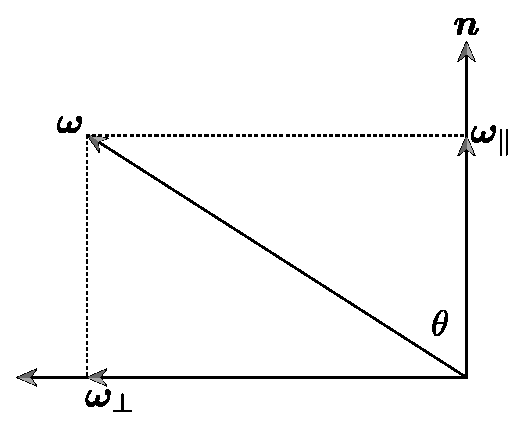
\includegraphics[width=0.4\linewidth]{Pictures/chap08/Parallelprojectionomeganormal.eps}
    \caption{向量$\bm\omega$在法线$\bm n$上的平行投影由${\bm\omega}_{\parallel}=(\cos\theta){\bm n}=({\bm n}\cdot{\bm\omega}){\bm n}$给出。
    垂直分量由${\bm\omega}_{\perp}=(\sin\theta){\bm n}$给出但用${\bm\omega}_{\perp}={\bm\omega}-{\bm\omega}_{\parallel}$计算更简单。}
    \label{fig:8.7}
\end{figure}

\reffig{8.8}展示了计算反射方向${\bm\omega}_{\mathrm{r}}$的设置。
我们可以看到两个向量都有相同的${\bm\omega}_{\parallel}$分量,
且${\bm\omega}_{\mathrm{r}\perp}$的值是${\bm\omega}_{\mathrm{o}\perp}$取反。
因此,我们有
\begin{align}
    \label{eq:8.5}
    {\bm\omega}_{\mathrm{r}}={\bm\omega}_{\mathrm{r}\perp}+{\bm\omega}_{\mathrm{r}\parallel} & =-{\bm\omega}_{\mathrm{o}\perp}+{\bm\omega}_{\mathrm{o}\parallel}\nonumber                                                        \\
                                                                                             & =-({\bm\omega}_{\mathrm{o}}-({\bm n}\cdot{\bm\omega}_{\mathrm{o}}){\bm n})+({\bm n}\cdot{\bm\omega}_{\mathrm{o}}){\bm n}\nonumber \\
                                                                                             & =-{\bm\omega}_{\mathrm{o}}+2({\bm n}\cdot{\bm\omega}_{\mathrm{o}}){\bm n}\, .
\end{align}
\begin{figure}[htbp]
    \centering
    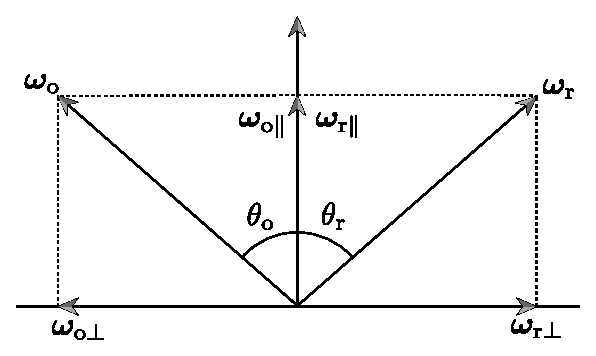
\includegraphics[width=0.5\linewidth]{Pictures/chap08/Perfectreflectioncomponents.eps}
    \caption{因为角$\theta_{\mathrm{o}}$和$\theta_{\mathrm{r}}$相等,
    所以完美反射方向的平行分量${\bm\omega}_{\mathrm{r}\parallel}$和
    入射方向的相同:${\bm\omega}_{\mathrm{r}\parallel}={\bm\omega}_{\mathrm{o}\parallel}$.
    其垂直分量就是入射方向垂直分量取反。}
    \label{fig:8.8}
\end{figure}

函数\refvar{Reflect}{()}实现了该计算。
\begin{lstlisting}
`\refcode{BSDF Inline Functions}{+=}\lastnext{BSDFInlineFunctions}`
inline `\refvar{Vector3f}{}` `\initvar{Reflect}{}`(const `\refvar{Vector3f}{}` &wo, const `\refvar{Vector3f}{}` &n) {
    return -wo + 2 * `\refvar{Dot}{}`(wo, n) * n;
}
\end{lstlisting}

在BRDF坐标系中,${\bm n}=(0,0,1)$,该表达式可极大简化。
\begin{lstlisting}
`\initcode{Compute perfect specular reflection direction}{=}`
*wi = `\refvar{Vector3f}{}`(-wo.x, -wo.y, wo.z);
\end{lstlisting}

\subsection{镜面透射}\label{sub:镜面透射}
我们现在推导镜面透射的BTDF。斯涅尔定律是推导的基础。
斯涅尔定律不仅给出了透射光线的方向,它还能用于说明
当光线穿过折射率不同的介质时,沿该光线的辐亮度会变。

考虑入射光线到达两种介质的边界,入射和出射介质的折射率
分别为$\eta_{\mathrm{i}}$和$\eta_{\mathrm{o}}$(\reffig{8.9})
\sidenote{译者注:原图把$\eta_{\mathrm{o}}$写成$\eta_{\mathrm{t}}$,
    与正文不一致,已修改。}。
\begin{figure}[htbp]
    \centering
    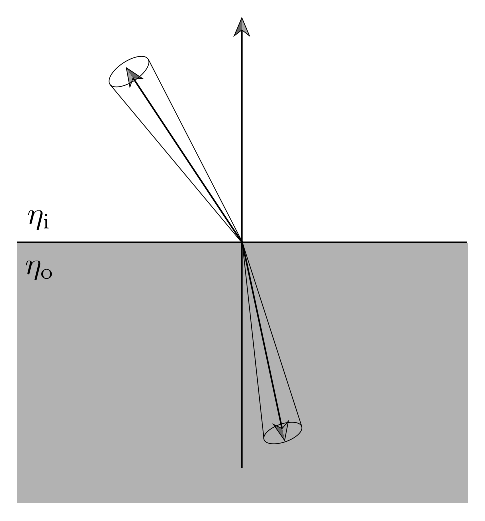
\includegraphics[width=0.5\linewidth]{Pictures/chap08/Radiancechangeatrefraction.eps}
    \caption{折射率不同的介质边界处透射辐亮度由这两个折射率之比的平方缩放。
        直观上这可以理解为辐射的微分立体角被压缩或展开作为透射的结果。}
    \label{fig:8.9}
\end{figure}

我们用$\tau$来表示菲涅尔方程给出的入射能量透射到出射方向的比例,
所以$\tau=1-F_{\mathrm{r}}({\bm\omega}_{\mathrm{i}})$.
于是透射的微分通量大小为
\begin{align*}
    \mathrm{d}\varPhi_{\mathrm{o}}=\tau\mathrm{d}\varPhi_{\mathrm{i}}\, .
\end{align*}
如果我们用辐亮度的定义\refeq{5.2},则我们有
\begin{align*}
    L_{\mathrm{o}}\cos\theta_{\mathrm{o}}\mathrm{d}A\mathrm{d}{\bm\omega}_{\mathrm{o}}=\tau(L_{\mathrm{i}}\cos\theta_{\mathrm{i}}\mathrm{d}A\mathrm{d}{\bm\omega}_{\mathrm{i}})\, .
\end{align*}
把立体角展开为球面角,我们有
\begin{align}
    \label{eq:8.6}
    L_{\mathrm{o}}\cos\theta_{\mathrm{o}}\mathrm{d}A\sin\theta_{\mathrm{o}}\mathrm{d}\theta_{\mathrm{o}}\mathrm{d}\varphi_{\mathrm{o}}=\tau L_{\mathrm{i}}\cos\theta_{\mathrm{i}}\mathrm{d}A\sin\theta_{\mathrm{i}}\mathrm{d}\theta_{\mathrm{i}}\mathrm{d}\varphi_{\mathrm{i}}\, .
\end{align}

我们现在可以对斯涅尔定律求$\theta$的微分,得到关系
\begin{align*}
    \eta_{\mathrm{o}}\cos\theta_{\mathrm{o}}\mathrm{d}\theta_{\mathrm{o}}=\eta_{\mathrm{i}}\cos\theta_{\mathrm{i}}\mathrm{d}\theta_{\mathrm{i}}\, .
\end{align*}
整理各项,我们有
\begin{align*}
    \frac{\cos\theta_{\mathrm{o}}\mathrm{d}\theta_{\mathrm{o}}}{\cos\theta_{\mathrm{i}}\mathrm{d}\theta_{\mathrm{i}}}=\frac{\eta_{\mathrm{i}}}{\eta_{\mathrm{o}}}\, .
\end{align*}
把该关系和斯涅尔定律代入\refeq{8.6}并化简,我们有
\begin{align*}
    L_{\mathrm{o}}\eta_{\mathrm{i}}^2\mathrm{d}\varphi_{\mathrm{o}}=\tau L_{\mathrm{i}}\eta_{\mathrm{o}}^2\mathrm{d}\varphi_{\mathrm{i}}\, .
\end{align*}
因为$\varphi_{\mathrm{i}}=\varphi_{\mathrm{o}}+\pi$,所以$\mathrm{d}\varphi_{\mathrm{i}}=\mathrm{d}\varphi_{\mathrm{o}}$,
我们有最终关系:
\begin{align}
    \label{eq:8.7}
    L_{\mathrm{o}}=\tau L_{\mathrm{i}}\frac{\eta_{\mathrm{o}}^2}{\eta_{\mathrm{i}}^2}\, .
\end{align}
对于镜面反射的BRDF,我们需要分离一个$\cos\theta_{\mathrm{i}}$项
来得到正确的镜面透射BTDF:
\begin{align*}
    f_{\mathrm{r}}({\bm\omega}_{\mathrm{o}},{\bm\omega}_{\mathrm{i}})=\frac{\eta_{\mathrm{o}}^2}{\eta_{\mathrm{i}}^2}(1-F_{\mathrm{r}}({\bm\omega}_{\mathrm{i}}))\frac{\delta({\bm\omega}_{\mathrm{i}}-T({\bm\omega}_{\mathrm{o}},{\bm n}))}{|\cos\theta_{\mathrm{i}|}}\, ,
\end{align*}
其中$T({\bm\omega}_{\mathrm{o}},{\bm n})$是
镜面透射${\bm\omega}_{\mathrm{o}}$穿过
曲面法线为$\bm n$的界面所得的镜面透射向量。

该方程中的项$1-F_{\mathrm{r}}({\bm\omega}_{\mathrm{i}})$对应了
容易观察到的效应:接近垂直的角度透射更强。例如,如果你直接朝下看着清澈的湖水,
你会看见水下深处,但角度平视时大部分光都像是镜子反射的。

类\refvar{SpecularTransmission}{}几乎和\refvar{SpecularReflection}{}一样,
除了采样方向是完美镜面透射的方向。\reffig{8.10}展示了使用
镜面反射和透射BRDF与BTDF来模拟玻璃的龙模型图像。
\begin{figure}[htbp]
    \centering
    \includegraphics[width=\linewidth]{Pictures/chap08/dragon-glass.png}
    \caption{当用菲涅尔公式调制了介电质的镜面反射BRDF和镜面透射BTDF,
        反射和透射量随角度的真实变化给出了玻璃在视觉上的准确表现
        (感谢Christian Schüller提供模型)。}
    \label{fig:8.10}
\end{figure}

\begin{lstlisting}
`\refcode{BxDF Declarations}{+=}\lastnext{BxDFDeclarations}`
class `\initvar{SpecularTransmission}{}` : public `\refvar{BxDF}{}` {
public:
    `\refcode{SpecularTransmission Public Methods}{}`
private:
    `\refcode{SpecularTransmission Private Data}{}`
};
\end{lstlisting}

\refvar{SpecularTransmission}{}的构造函数保存了曲面两侧的折射率,
其中{\ttfamily etaA}是曲面上方的折射率(这里曲面法线所在的一侧为“上方”),
{\ttfamily etaB}是曲面下方的折射率,而{\ttfamily T}给出了透射缩放因子。
参数\refvar{TransportMode}{}表示入射光线交点的\refvar{BxDF}{}是
从光源还是相机开始计算的。该区别指出了该怎样计算\refvar{BxDF}{}的作用。
\begin{lstlisting}
`\initcode{SpecularTransmission Public Methods}{=}\initnext{SpecularTransmissionPublicMethods}`
`\refvar{SpecularTransmission}{}`(const `\refvar{Spectrum}{}` &T, `\refvar{Float}{}` etaA, `\refvar{Float}{}` etaB,
        `\refvar{TransportMode}{}` mode) 
    : `\refvar{BxDF}{}`(`\refvar{BxDFType}{}`(`\refvar[BSDFTRANSMISSION]{BSDF\_TRANSMISSION}{}` | `\refvar[BSDFSPECULAR]{BSDF\_SPECULAR}{}`)), `\refvar[SpecularTransmission::T]{T}{}`(T), `\refvar[SpecularTransmission::etaA]{etaA}{}`(etaA),
      `\refvar[SpecularTransmission::etaB]{etaB}{}`(etaB), `\refvar[SpecularTransmission::fresnel]{fresnel}{}`(etaA, etaB), `\refvar[SpecularTransmission::mode]{mode}{}`(mode) {
}
\end{lstlisting}
因为导体不透射光,所以\refvar{FresnelDielectric}{}对象
总是用于菲涅尔计算。

\begin{lstlisting}
`\initcode{SpecularTransmission Private Data}{=}`
const `\refvar{Spectrum}{}` `\initvar[SpecularTransmission::T]{T}{}`;
const `\refvar{Float}{}` `\initvar[SpecularTransmission::etaA]{etaA}{}`, `\initvar[SpecularTransmission::etaB]{etaB}{}`;
const `\refvar{FresnelDielectric}{}` `\initvar[SpecularTransmission::fresnel]{fresnel}{}`;
const `\refvar{TransportMode}{}` `\initvar[SpecularTransmission::mode]{mode}{}`;
\end{lstlisting}

对于\refvar{SpecularReflection}{},因为BTDF是缩放后的$\delta$分布,所以\linebreak
\refvar{SpecularTransmission::f}{()}总是返回零。
\begin{lstlisting}
`\refcode{SpecularTransmission Public Methods}{+=}\lastnext{SpecularTransmissionPublicMethods}`
`\refvar{Spectrum}{}` `\initvar[SpecularTransmission::f]{f}{}`(const `\refvar{Vector3f}{}` &wo, const `\refvar{Vector3f}{}` &wi) const { 
    return `\refvar{Spectrum}{}`(0.f); 
}
\end{lstlisting}

\refeq{8.7}描述了当光线从一种介质进入另一种时辐亮度是怎样变化的。
然而事实证明,尽管该缩放应该应用于从光源开始的光线,
但\emph{绝不}该用于从相机开始的光线。
\refsec{路径-空间测量方程}将更细致地讨论该问题以及到时候定义的运用该缩放的
代码片{\refcode{Account for non-symmetry with transmission to different medium}{}}。
\begin{lstlisting}
`\refcode{BxDF Method Definitions}{+=}\lastnext{BxDFMethodDefinitions}`
`\refvar{Spectrum}{}` `\refvar{SpecularTransmission}{}`::`\initvar[SpecularTransmission::Samplef]{Sample\_f}{}`(const `\refvar{Vector3f}{}` &wo,
        `\refvar{Vector3f}{}` *wi, const `\refvar{Point2f}{}` &sample, `\refvar{Float}{}` *pdf,
        `\refvar{BxDFType}{}` *sampledType) const {
    `\refcode{Figure out which $\eta$ is incident and which is transmitted}{}`
    `\refcode{Compute ray direction for specular transmission}{}`
    *pdf = 1;
    `\refvar{Spectrum}{}` ft = `\refvar[SpecularTransmission::T]{T}{}` * (`\refvar{Spectrum}{}`(1.) - `\refvar[SpecularTransmission::fresnel]{fresnel}{}`.`\refvar[FresnelDielectric::Evaluate]{Evaluate}{}`(`\refvar{CosTheta}{}`(*wi)));
    `\refcode{Account for non-symmetry with transmission to different medium}{}`
    return ft / `\refvar{AbsCosTheta}{}`(*wi);
}
\end{lstlisting}

该方法首先确定入射光线是否正进入或退出折射介质。
pbrt遵循局部反射空间中的曲面法线即$(0,0,1)$方向指向
物体外侧的惯例。因此,如果方向${\bm\omega_{\mathrm{o}}}$的$z$分量
大于零,则入射光线来自物体外侧。
\begin{lstlisting}
`\initcode{Figure out which $\eta$ is incident and which is transmitted}{=}`
bool entering = `\refvar{CosTheta}{}`(wo) > 0;
`\refvar{Float}{}` etaI = entering ? `\refvar[SpecularTransmission::etaA]{etaA}{}` : `\refvar[SpecularTransmission::etaB]{etaB}{}`;
`\refvar{Float}{}` etaT = entering ? `\refvar[SpecularTransmission::etaB]{etaB}{}` : `\refvar[SpecularTransmission::etaA]{etaA}{}`;
\end{lstlisting}
\begin{lstlisting}
`\initcode{Compute ray direction for specular transmission}{=}`
if (!`\refvar{Refract}{}`(wo, `\refvar{Faceforward}{}`(`\refvar{Normal3f}{}`(0, 0, 1), wo), etaI / etaT, wi))
    return 0;
\end{lstlisting}

为了推导给出透射方向向量的表达式,我们可以采用
类似于我们为镜面反射所用的更简单的方法。
\reffig{8.11}展示了该设置。

\begin{figure}[htbp]
    \centering
    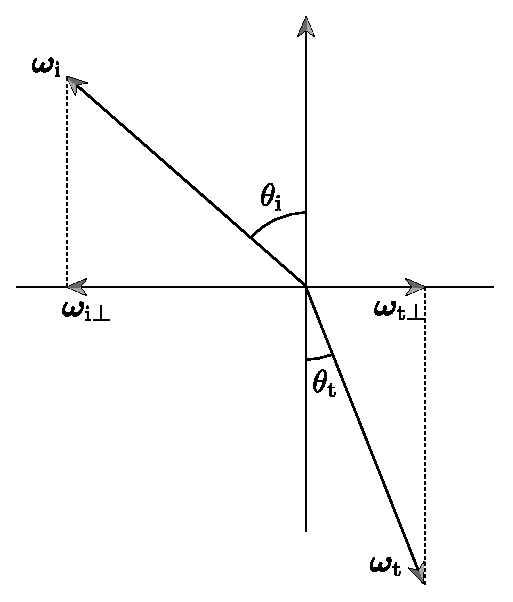
\includegraphics[width=0.5\linewidth]{Pictures/chap08/Speculartransmissionprojections.eps}
    \caption{镜面透射的几何结构。给定入射方向${\bm\omega}_{\mathrm{i}}$和
        曲面法线$\bm n$间的夹角$\theta_{\mathrm{i}}$,镜面透射方向与
        曲面法线成角为$\theta_{\mathrm{t}}$. 该方向${\bm\omega}_{\mathrm{t}}$可
        用斯涅尔定律算得,即求其垂直分量${\bm\omega}_{\mathrm{t}\perp}$,
        再算${\bm\omega}_{\mathrm{t}\parallel}$得到规范化结果${\bm\omega}_{\mathrm{t}}$.}
    \label{fig:8.11}
\end{figure}

然而这次,我们将从垂直分量开始:如果入射向量规范化了且有
垂直分量${\bm\omega}_{\mathrm{i}\perp}$,则我们从三角学
以及${\bm\omega}_{\perp}$的定义中知道${\bm\omega}_{\mathrm{i}\perp}$的长度
等于$\sin\theta_{\mathrm{i}}$. 斯涅尔定律告诉
我们$\displaystyle\sin\theta_{\mathrm{t}}=\frac{\eta_{\mathrm{i}}}{\eta_{\mathrm{t}}}\sin\theta_{\mathrm{i}}$.
让方向${\bm\omega}_{\mathrm{i}\perp}$取反并相应调整长度,我们有
\begin{align*}
    {\bm\omega}_{\mathrm{t}\perp}=\frac{\eta_{\mathrm{i}}}{\eta_{\mathrm{t}}}(-{\bm\omega}_{\mathrm{i}\perp})\, .
\end{align*}
等价地,因为${\bm\omega}_{\perp}={\bm\omega}-{\bm\omega}_{\parallel}$,
\begin{align*}
    {\bm\omega}_{\mathrm{t}\perp}=\frac{\eta_{\mathrm{i}}}{\eta_{\mathrm{t}}}(-{\bm\omega}_{\mathrm{i}}+({\bm\omega}_{\mathrm{i}}\cdot{\bm n}){\bm n})\, .
\end{align*}

现在对于${\bm\omega}_{\mathrm{t}\parallel}$:我们
知道${\bm\omega}_{\mathrm{t}\parallel}$平行于$\bm n$但面向相反方向,
且我们还知道${\bm\omega}_{\mathrm{t}}$应该规范化。把这些合起来,
\begin{align*}
    {\bm\omega}_{\mathrm{t}\parallel}=-\left(\sqrt{1-\|{\bm\omega}_{\mathrm{t}\perp}\|^2}\right){\bm n}\, .
\end{align*}
于是完整的向量${\bm\omega}_{\mathrm{t}}$是
\begin{align*}
    {\bm\omega}_{\mathrm{t}}={\bm\omega}_{\mathrm{t}\perp}+{\bm\omega}_{\mathrm{t}\parallel}=\frac{\eta_{\mathrm{i}}}{\eta_{\mathrm{t}}}(-{\bm\omega}_{\mathrm{i}})+\left[\frac{\eta_{\mathrm{i}}}{\eta_{\mathrm{t}}}({\bm\omega}_{\mathrm{i}}\cdot{\bm n})-\sqrt{1-\|{\bm\omega}_{\mathrm{t}\perp}\|^2}\right]{\bm n}\, .
\end{align*}
因为$\|{\bm\omega}_{\mathrm{t}\perp}\|=\sin\theta_{\mathrm{t}}$,
平方根下的项为$1-\sin^2\theta_{\mathrm{t}}=\cos^2\theta_{\mathrm{t}}$,
这给出了最终结果:
\begin{align}
    \label{eq:8.8}
    {\bm\omega}_{\mathrm{t}}=\frac{\eta_{\mathrm{i}}}{\eta_{\mathrm{t}}}(-{\bm\omega}_{\mathrm{i}})+\left[\frac{\eta_{\mathrm{i}}}{\eta_{\mathrm{t}}}({\bm\omega}_{\mathrm{i}}\cdot{\bm n})-\cos\theta_{\mathrm{t}}\right]{\bm n}\, .
\end{align}

分别给定入射方向{\ttfamily wi}、和{\ttfamily wi}在同一半球的
曲面法线{\ttfamily n}以及入射和透射介质折射率之比{\ttfamily eta},
函数\refvar{Refract}{()}计算折射方向{\ttfamily wt}。
布尔返回值表示{\ttfamily *wt}中是否返回了有效的折射光线;
全内反射情况下它取{\ttfamily false}。
\begin{lstlisting}
`\refcode{BSDF Inline Functions}{+=}\lastnext{BSDFInlineFunctions}`
inline bool `\initvar{Refract}{}`(const `\refvar{Vector3f}{}` &wi, const `\refvar{Normal3f}{}` &n, `\refvar{Float}{}` eta,
        `\refvar{Vector3f}{}` *wt) {
    `\refcode{Compute cos $\theta_t$ using Snell's law}{}`
    *wt = eta * -wi + (eta * cosThetaI - cosThetaT) * `\refvar{Vector3f}{}`(n);
    return true;
}
\end{lstlisting}

让斯涅尔定律两边平方能让我们计算$\cos\theta_{\mathrm{t}}$:
\begin{align*}
    \eta_{\mathrm{i}}^2\sin^2\theta_{\mathrm{i}} & =\eta_{\mathrm{t}}^2\sin^2\theta_{\mathrm{t}}\, ,                                      \\
    \sin^2\theta_{\mathrm{t}}                    & =\frac{\eta_{\mathrm{i}}^2}{\eta_{\mathrm{t}}^2}\sin^2\theta_{\mathrm{i}}\, ,          \\
    1-\cos^2\theta_{\mathrm{t}}                  & =\frac{\eta_{\mathrm{i}}^2}{\eta_{\mathrm{t}}^2}\sin^2\theta_{\mathrm{i}}\, ,          \\
    \cos\theta_{\mathrm{t}}                      & =\sqrt{1-\frac{\eta_{\mathrm{i}}^2}{\eta_{\mathrm{t}}^2}\sin^2\theta_{\mathrm{i}}}\, .
\end{align*}

\begin{lstlisting}
`\initcode{Compute cos $\theta_t$ using Snell's law}{=}`
`\refvar{Float}{}` cosThetaI = `\refvar{Dot}{}`(n, wi);
`\refvar{Float}{}` sin2ThetaI = std::max(0.f, 1.f - cosThetaI * cosThetaI);
`\refvar{Float}{}` sin2ThetaT = eta * eta * sin2ThetaI;
`\refcode{Handle total internal reflection for transmission}{}`
`\refvar{Float}{}` cosThetaT = std::sqrt(1 - sin2ThetaT);
\end{lstlisting}

我们这里也需要处理全内反射的情况。
如果$\sin\theta_{\mathrm{t}}$的平方值大于或等于一,
就发生了全内反射,所以返回{\ttfamily false}
\footnote{第一版pbrt在这里测试的“>1”而不是“>=1”。
    尽管两者的区别看起来无害,但该差异使得偶尔会算出not-a-number值,
    因为$\omega$(在曲面切平面上)的$z$分量为零,进而项$\frac{1}{\cos\theta}$为无穷。}。
\begin{lstlisting}
`\initcode{Handle total internal reflection for transmission}{=}`
if (sin2ThetaT >= 1) return false;
\end{lstlisting}

\subsection{菲涅尔调制的镜面反射与透射}\label{sub:菲涅尔调制的镜面反射与透射}
为了后续第\refchap{光传输I:表面反射}、
\refchap{光传输II:体积渲染}、\refchap{光传输III:双向方法}的
一些蒙特卡罗光传输算法有更优的效率,拥有能同时表示
镜面反射与镜面透射的单个\refvar{BxDF}{}很有用,
其中散射类型的相对权重由介电质菲涅尔方程调制。
\refvar{FresnelSpecular}{}中提供了这样的\refvar{BxDF}{}。
\begin{lstlisting}
`\refcode{BxDF Declarations}{+=}\lastnext{BxDFDeclarations}`
class `\initvar{FresnelSpecular}{}` : public `\refvar{BxDF}{}` {
public:
    `\refcode{FresnelSpecular Public Methods}{}`
private:
    `\refcode{FresnelSpecular Private Data}{}`
};
\end{lstlisting}
\begin{lstlisting}
`\initcode{FresnelSpecular Public Methods}{=}\initnext{FresnelSpecularPublicMethods}`
`\refvar{FresnelSpecular}{}`(const `\refvar{Spectrum}{}` &R, const `\refvar{Spectrum}{}` &T, `\refvar{Float}{}` etaA,
        `\refvar{Float}{}` etaB, `\refvar{TransportMode}{}` mode) 
    : `\refvar{BxDF}{}`(`\refvar{BxDFType}{}`(`\refvar[BSDFREFLECTION]{BSDF\_REFLECTION}{}` | `\refvar[BSDFTRANSMISSION]{BSDF\_TRANSMISSION}{}` | `\refvar[BSDFSPECULAR]{BSDF\_SPECULAR}{}`)),
      `\refvar[FresnelSpecular::R]{R}{}`(R), `\refvar[FresnelSpecular::T]{T}{}`(T), `\refvar[FresnelSpecular::etaA]{etaA}{}`(etaA), `\refvar[FresnelSpecular::etaB]{etaB}{}`(etaB), `\refvar[FresnelSpecular::fresnel]{fresnel}{}`(etaA, etaB),
      `\refvar[FresnelSpecular::mode]{mode}{}`(mode) { }
\end{lstlisting}

因为我们只关注介电质情形,所以\refvar{FresnelDielectric}{}对象
总是只用于菲涅尔计算。

\begin{lstlisting}
`\initcode{FresnelSpecular Private Data}{=}`
const `\refvar{Spectrum}{}` `\initvar[FresnelSpecular::R]{R}{}`, `\initvar[FresnelSpecular::T]{T}{}`;
const `\refvar{Float}{}` `\initvar[FresnelSpecular::etaA]{etaA}{}`, `\initvar[FresnelSpecular::etaB]{etaB}{}`;
const `\refvar{FresnelDielectric}{}` `\initvar[FresnelSpecular::fresnel]{fresnel}{}`;
const `\refvar{TransportMode}{}` `\initvar[FresnelSpecular::mode]{mode}{}`
\end{lstlisting}
\begin{lstlisting}
`\refcode{FresnelSpecular Public Methods}{+=}\lastcode{FresnelSpecularPublicMethods}`
`\refvar{Spectrum}{}` `\initvar[FresnelSpecular::f]{f}{}`(const `\refvar{Vector3f}{}` &wo, const `\refvar{Vector3f}{}` &wi) const { 
    return `\refvar{Spectrum}{}`(0.f); 
}
\end{lstlisting}

因为一些实现细节依赖于第\refchap{蒙特卡罗积分}介绍的蒙特卡罗积分原理,
方法\refvar[FresnelSpecular::Samplef]{Sample\_f}{()}
的实现在\refsub{镜面反射与透射}。